\documentclass{beamer}
\usepackage[utf8]{inputenc}
\usepackage{graphicx}

% Remove navigation controls
\usenavigationsymbolstemplate{}

% Slide numbering
\setbeamertemplate{footline}[frame number]

\title{Integrity checking in RDF databases using SPARQL constraints}
\subtitle{
  A brief introduction to the subject of my training period
}
\author{
  Leandro Lovisolo
}
\date{September 11, 2015}
\institute{
  I.N.R.A. SupAgro \\
  Montpellier, France
}

\begin{document}

\begin{frame}
  \titlepage
\end{frame}

\begin{frame}
  \frametitle{Motivation}
  \framesubtitle{Problem statement}

  \pause

  \begin{itemize}
    \item We're trying to answer questions that require consulting
      heterogeneous data sources.

    \pause

    \begin{itemize}
      \item Literature with inconsistent, semi-structured data.

      \pause

      \item No standard naming convention.

      \pause

      \item No information about the reliability of the data sources.

      \pause

      \item Each data source has its specific browsing/querying mechanism (no
        common interface.)
    \end{itemize}
  \end{itemize}
\end{frame}

\begin{frame}
  \frametitle{Motivation}
  \framesubtitle{Sample problem domain: \textbf{biorefinery}}

  \begin{itemize}
    \item Ligno-cellulosic biomass pre-treatment before enzymatic hydrolysis is
      an essential step to obtain good yields.

    \pause

    \item Several pre-treatment principles available, but \textbf{no clear
      criteria on how to choose the best one} taking into account environmental
      sustainability for a given biomass and biorefinery product (e.g.
      glucose.)
  \end{itemize}
\end{frame}

\begin{frame}
  \frametitle{Motivation}
  \framesubtitle{Sample problem domain: \textbf{packaging selection}}

  TODO
\end{frame}

\begin{frame}
  \frametitle{Proposed solution}

  \begin{itemize}
    \item Represent scientific knowledge with ontologies using recommended
      standardized tools and languages for such purposes (semantic web
      technologies, RDF(S), OWL, etc.)

    \pause

    \item Develop an ontology and data management web application (e.g. the
      \textbf{@Web platform}) that makes it easy for scientists to introduce
      data from scientific publications into an ontology, execute queries
      against an ontology, etc.

    \pause

    \item Create integrity constraints to automatically detect inconsistencies
      and errors in scientific publications and to automatically classify
      publications according to their topics.

    \pause

    \begin{itemize}
      \item The focus of my internship!
    \end{itemize}

  \end{itemize}
\end{frame}

\begin{frame}
  \frametitle{An example of a termino-ontological resource}
  \framesubtitle{Taken from the biorefinery application}

  \begin{center}
    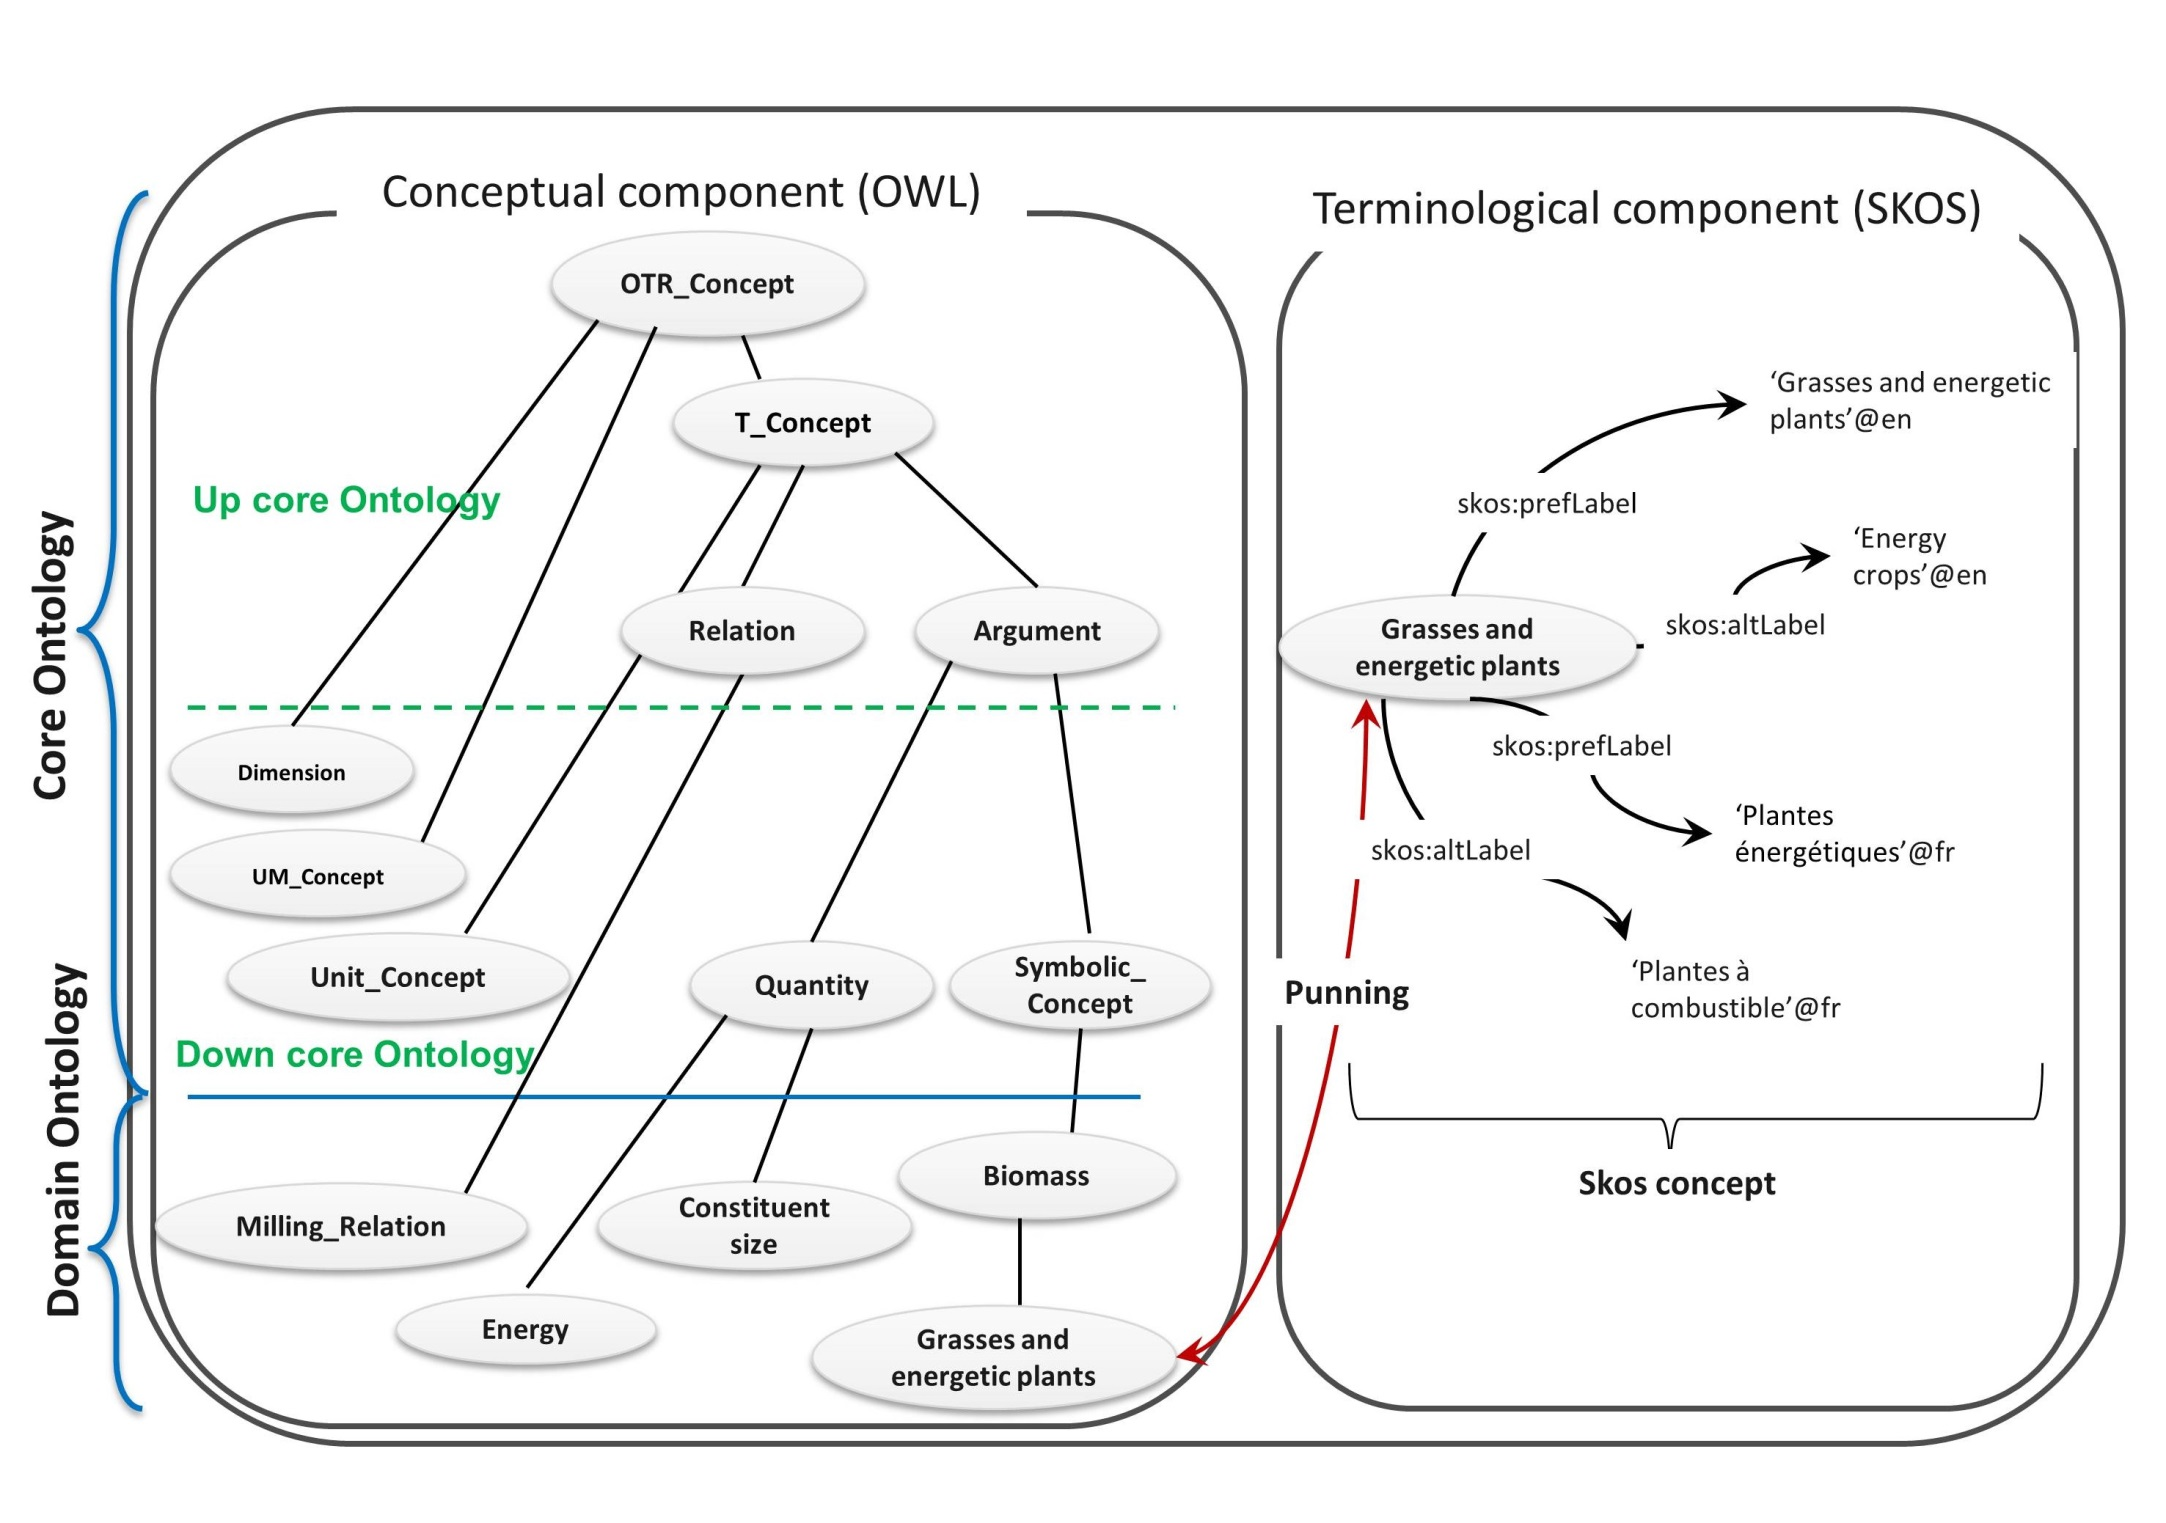
\includegraphics[width=10cm]{termino-ontological-resource.jpg}
  \end{center}
\end{frame}

\begin{frame}
  \frametitle{Design goals for the core ontology}

  \begin{itemize}
    \item \textbf{Simple} so as to make the annotator's task easier.

    \pause

    \item \textbf{Generic} enough so that the approach can be applied to
      different, unrelated domains.

    \pause

    \begin{itemize}
      \item Proven in the domains of biorefinery and packaging selection.
    \end{itemize}
  \end{itemize}
\end{frame}

\begin{frame}
  \frametitle{A sample relation}
  \framesubtitle{Also from the biorefinery domain}

  \begin{center}
    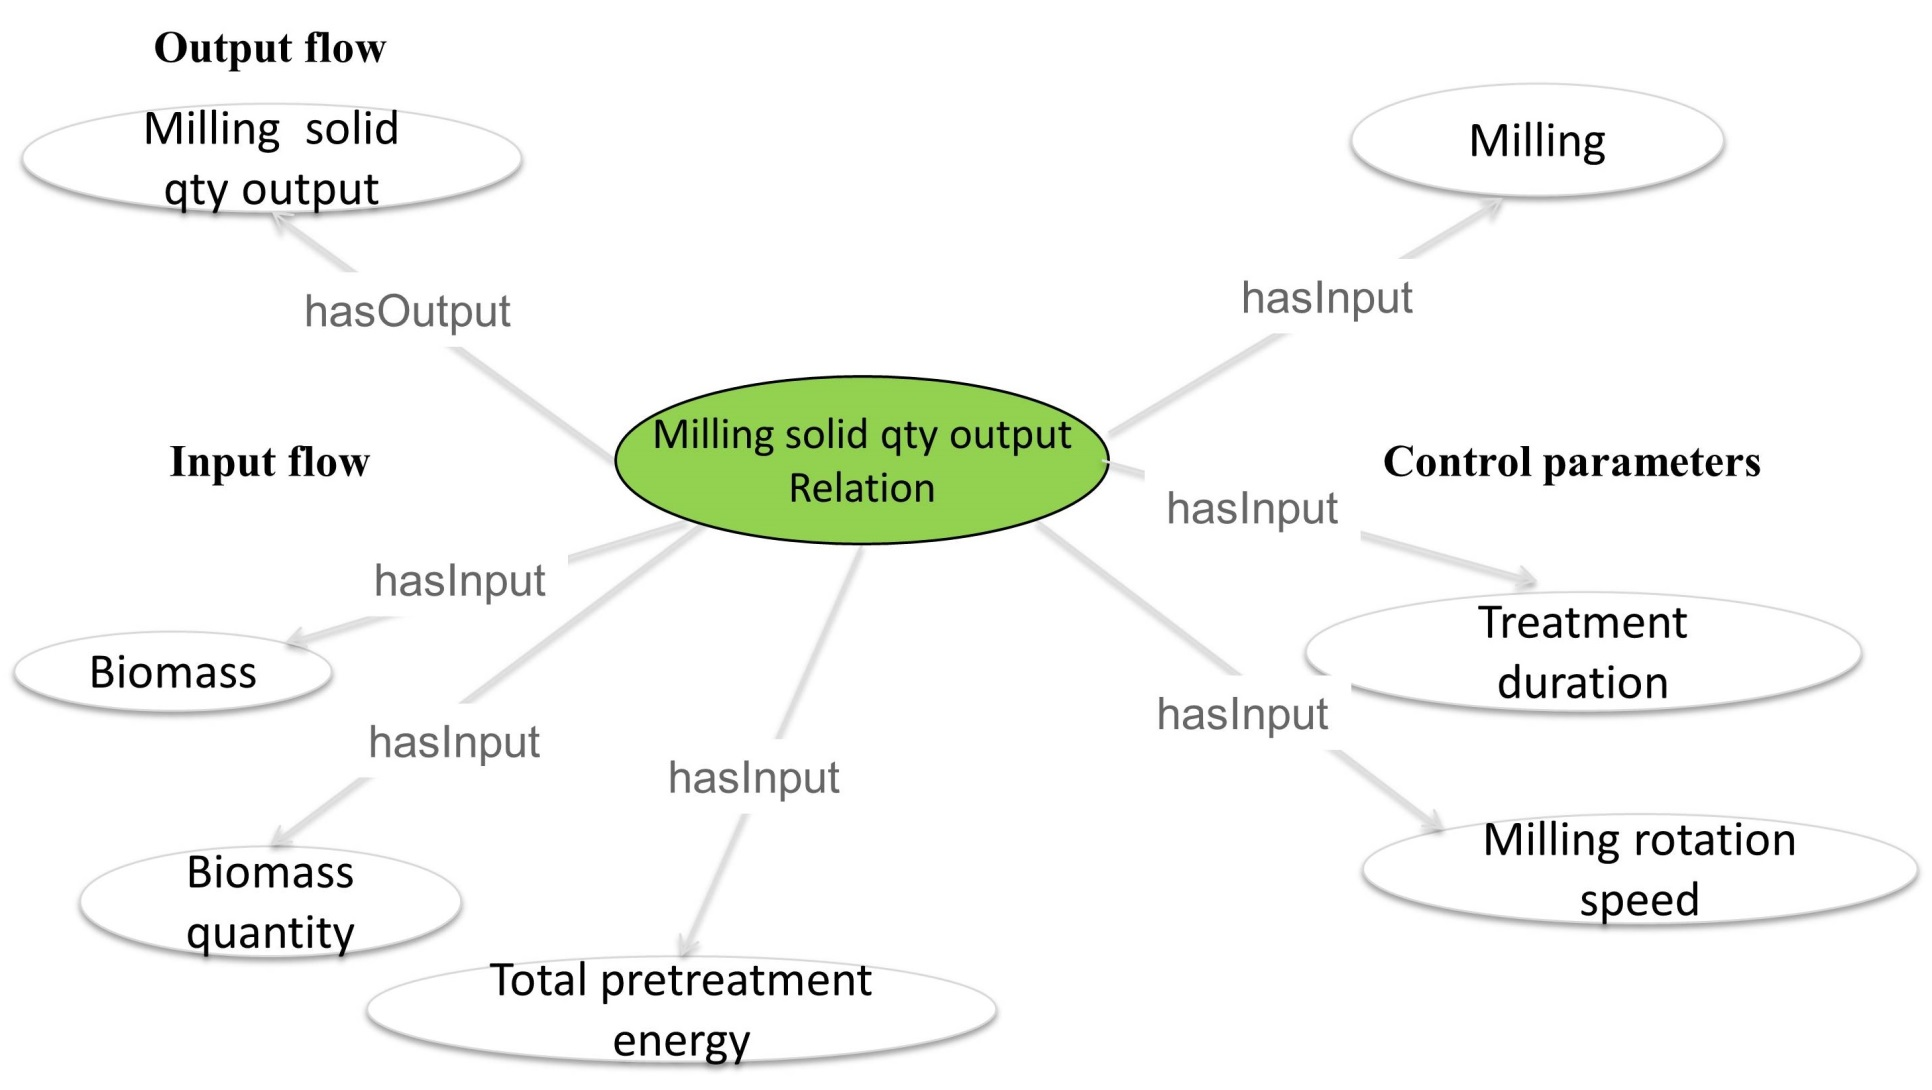
\includegraphics[width=10cm]{relation.jpg}
  \end{center}
\end{frame}

\begin{frame}
  \frametitle{The \textbf{@Web} platform}
  \framesubtitle{Exploring an ontology}

  \begin{center}
    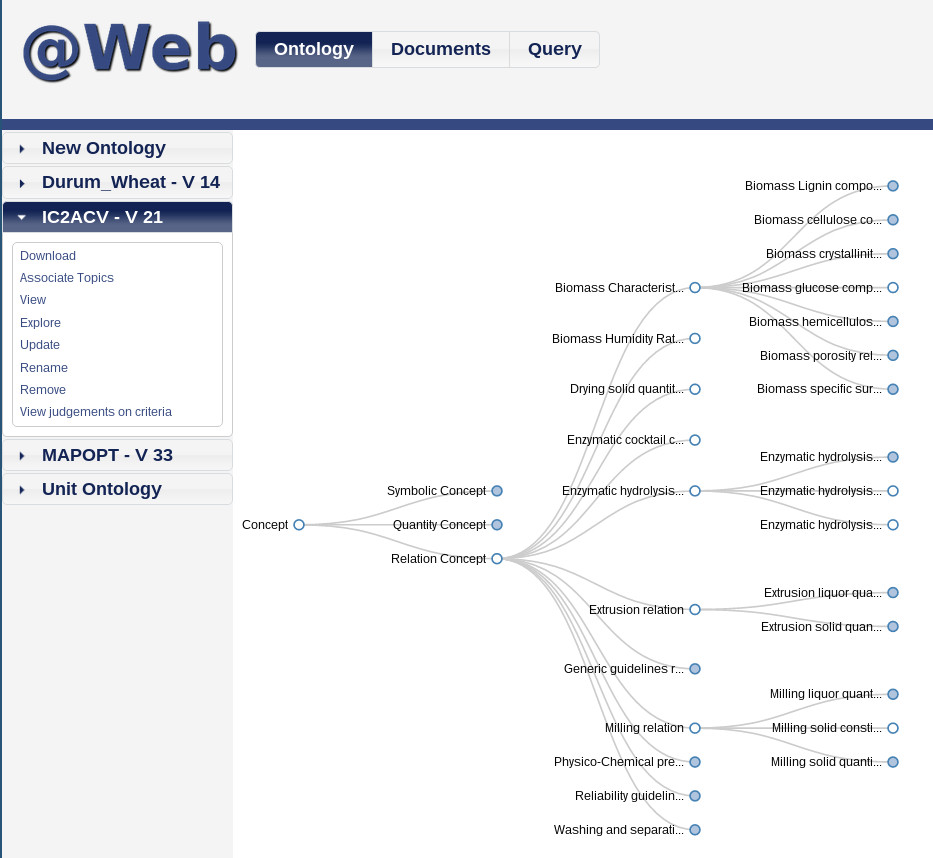
\includegraphics[width=8cm]{atweb-ontology.jpg}
  \end{center}
\end{frame}

\begin{frame}
  \frametitle{The \textbf{@Web} platform}
  \framesubtitle{Browsing documents}

  \begin{center}
    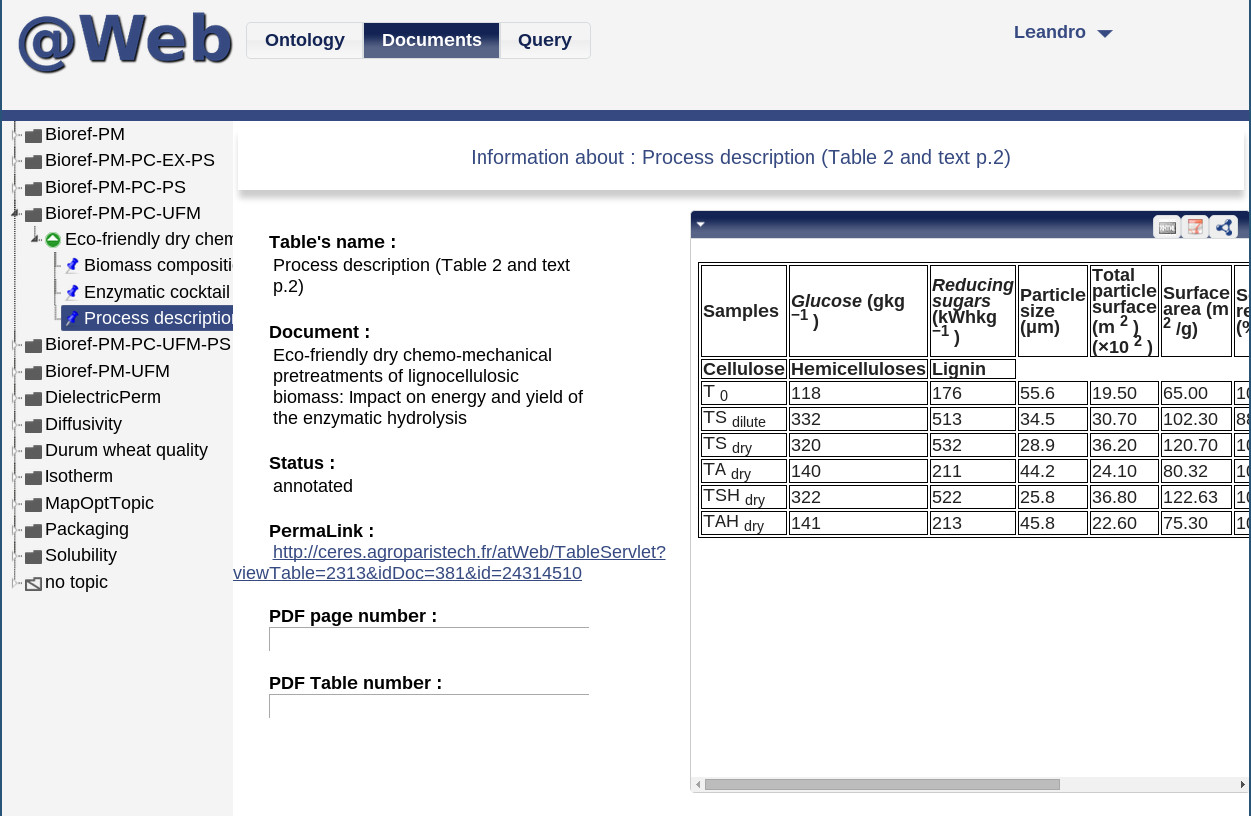
\includegraphics[width=10cm]{atweb-document.jpg}
  \end{center}
\end{frame}

\begin{frame}
  \frametitle{The \textbf{@Web} platform}
  \framesubtitle{Querying an ontology: defining the search scope}

  \begin{center}
    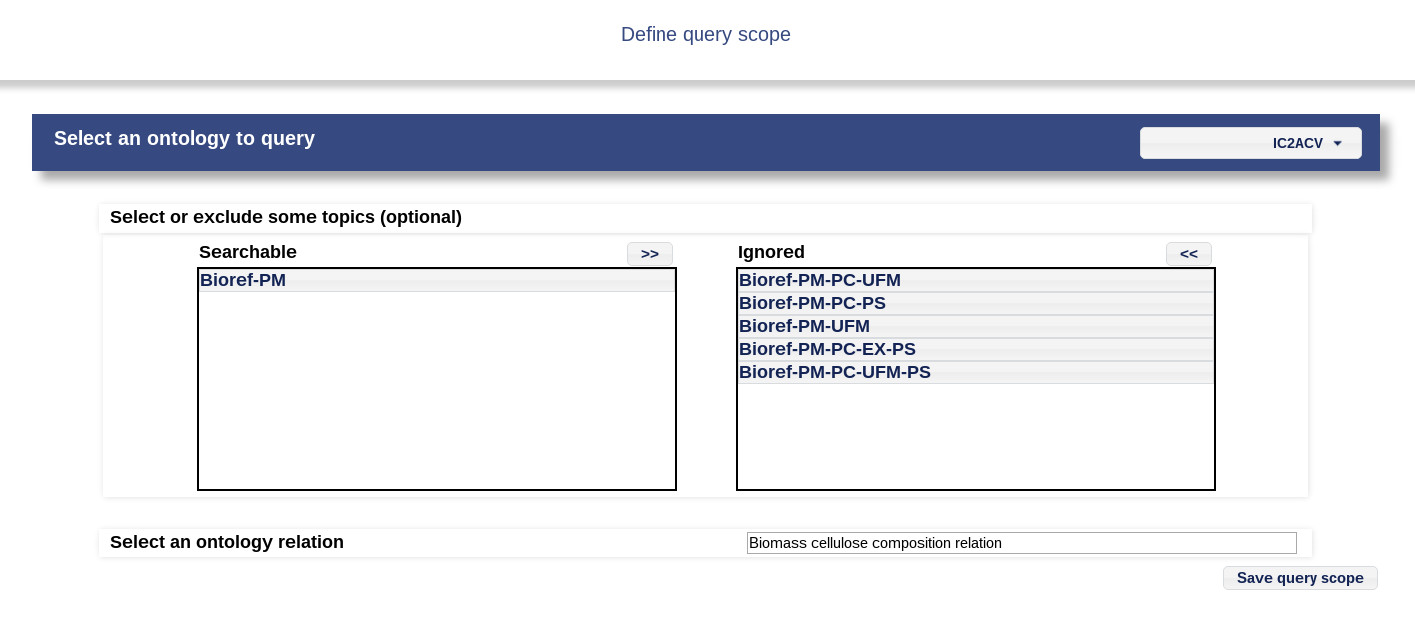
\includegraphics[width=10cm]{atweb-query-1.jpg}
  \end{center}
\end{frame}

\begin{frame}
  \frametitle{The \textbf{@Web} platform}
  \framesubtitle{Querying an ontology: search parameters}

  \begin{center}
    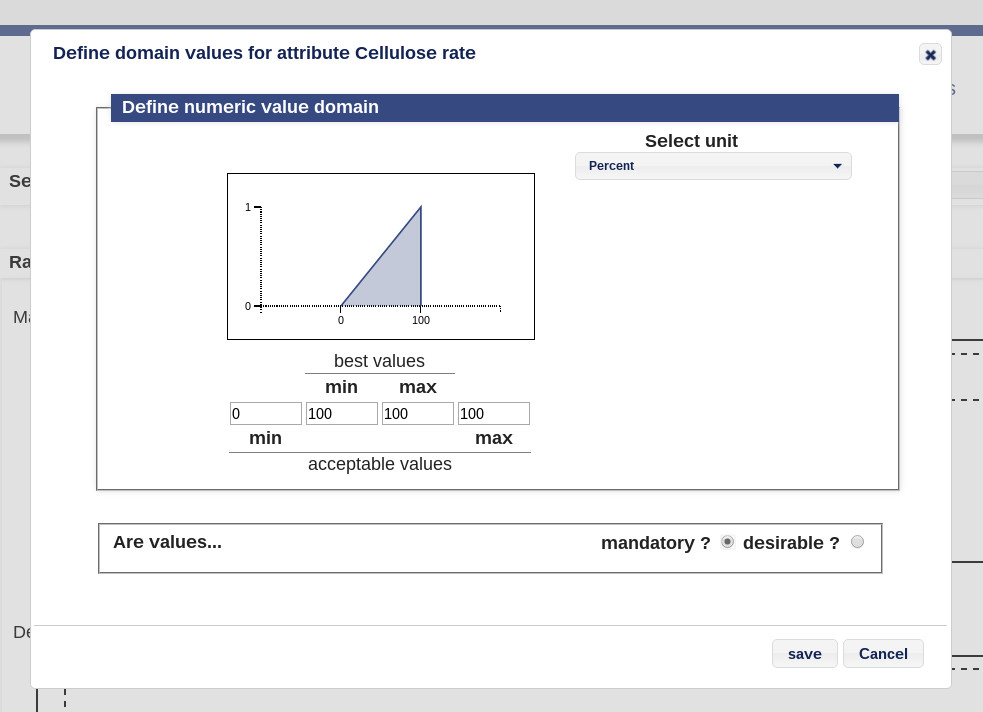
\includegraphics[width=10cm]{atweb-query-2.jpg}
  \end{center}
\end{frame}

\begin{frame}
  \frametitle{The \textbf{@Web} platform}
  \framesubtitle{Querying an ontology: executing a query}

  \begin{center}
    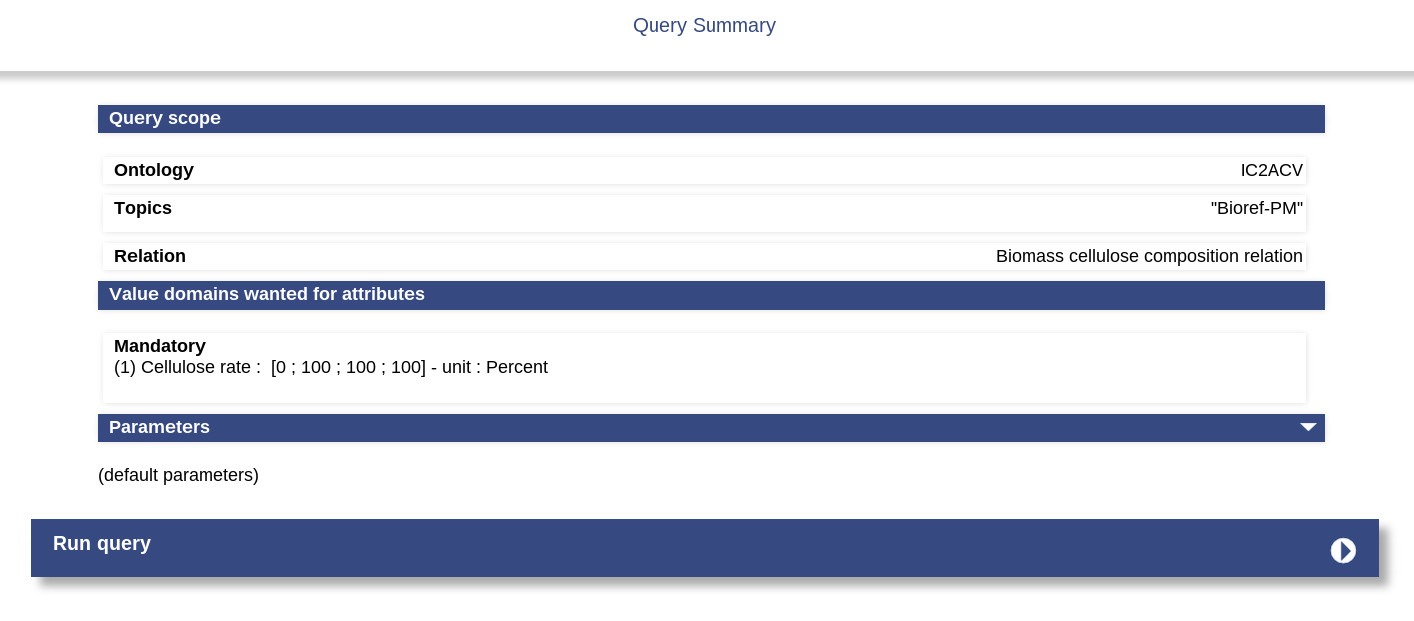
\includegraphics[width=10cm]{atweb-query-3.jpg}
  \end{center}
\end{frame}

\begin{frame}
  \frametitle{The \textbf{@Web} platform}
  \framesubtitle{Querying an ontology: results}

  \begin{center}
    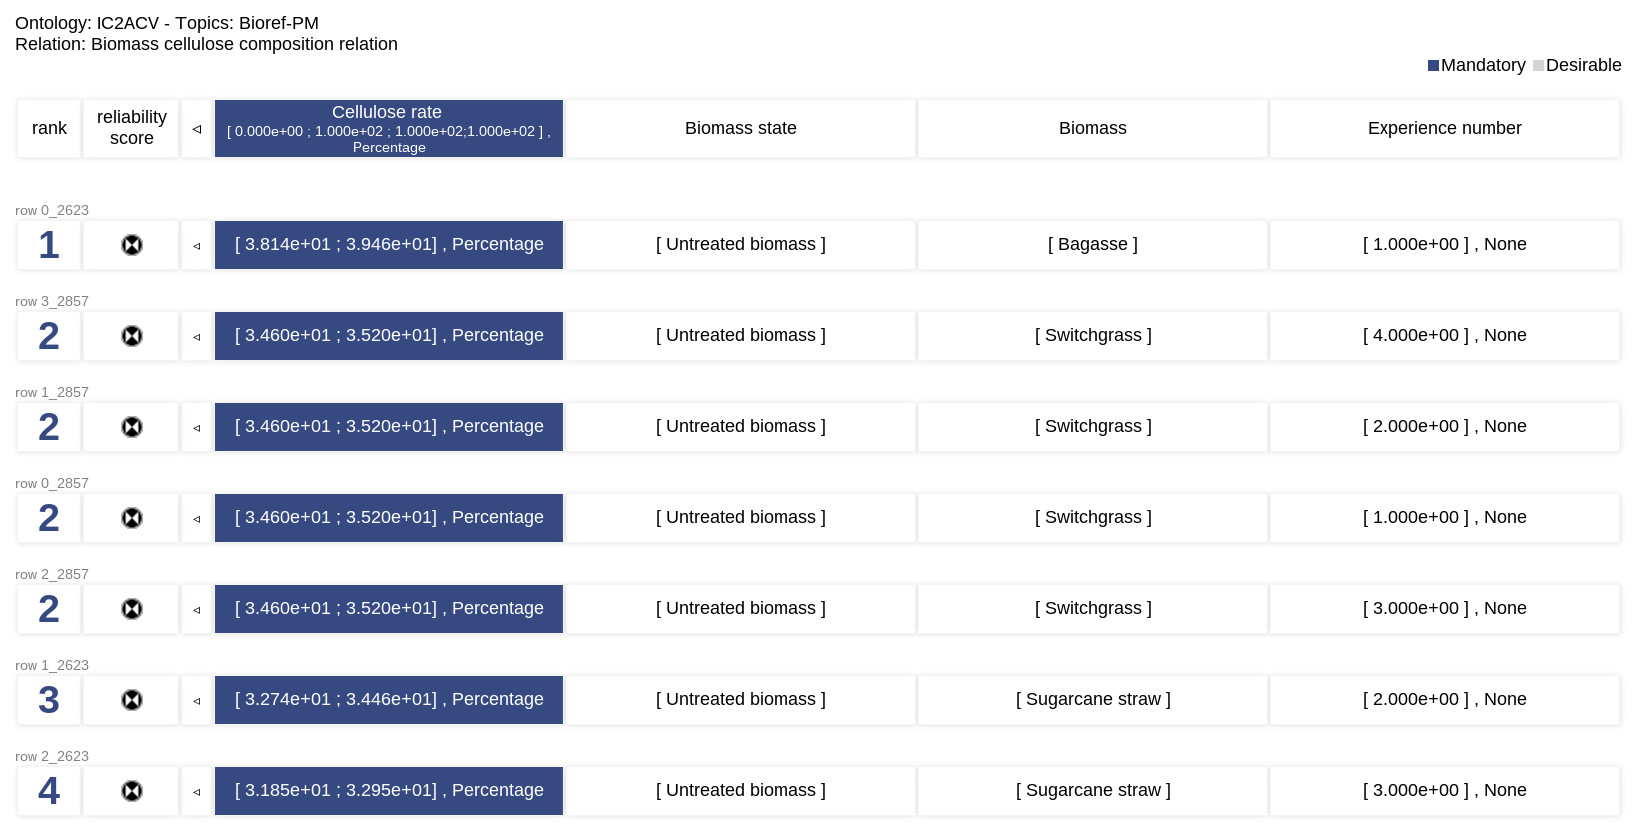
\includegraphics[width=10cm]{atweb-query-4.jpg}
  \end{center}
\end{frame}

\begin{frame}
  \frametitle{The annotator's task}

  \begin{itemize}
    \item Given a scientific publication and a desired ontology, capture data
      from the publication using the appropriate concepts in the ontology.

    \pause

    \item Create and update concepts in the ontology as they're discovered
      during the annotation process (i.e. in an iterative fashion.)

    \pause

    \item Write and edit \textbf{guidelines} associated to each concept
      explaining when and how a concept should be used.
  \end{itemize}
\end{frame}

\begin{frame}
  \frametitle{An example of data captured from a scientific publication}

  TODO: Find a better example.

  \begin{center}
    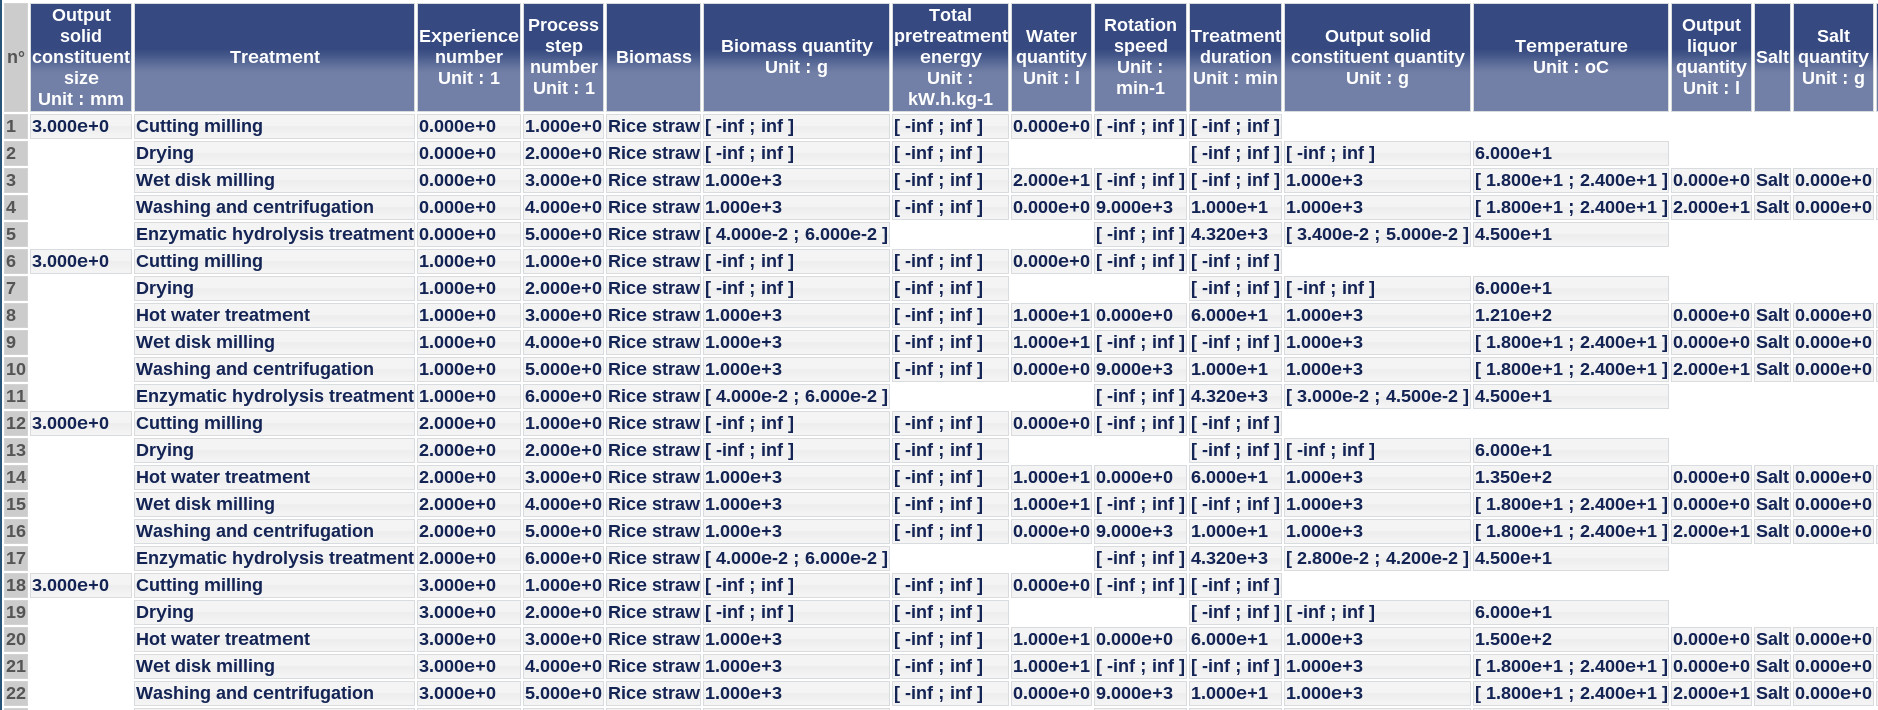
\includegraphics[width=11cm]{table.jpg}
  \end{center}
\end{frame}

\begin{frame}
  \frametitle{A sample guideline}

  \begin{center}
    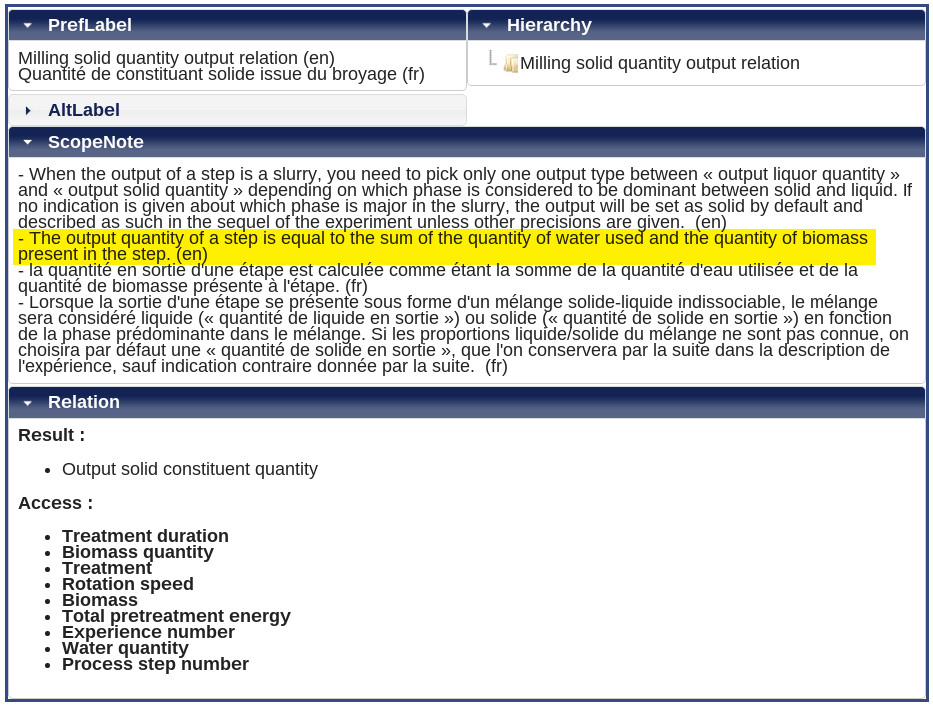
\includegraphics[width=10cm]{guideline.jpg}
  \end{center}
\end{frame}

\begin{frame}
  \frametitle{Some sample guidelines that can be easily translated into SPARQL
  constraints}
  \framesubtitle{Integrity constraints}

  \begin{itemize}
    \item \textit{``The output quantity of a step is equal to the sum of the
      quantity of water used and the quantity of biomass present in the
    step.''}

    \pause

    \item \textit{``When the biomass doesn't have starch, we consider that the
      cellulose percentage equals to the glucose percentage and that the
    hemicellulose percentage equals to the sum of xylose and arabinose
  percentage (and potential other sugars like mannose, galactose, etc.)''}

    \pause

    \item \textit{``Furthermore, we consider that the glucose rate equals to
      glucan rate divided by 0.9.''}
  \end{itemize}
\end{frame}

\begin{frame}
  \frametitle{Some sample guidelines that can be easily translated into SPARQL
  constraints}
  \framesubtitle{Classification constraints}

  TODO
\end{frame}

\begin{frame}
  \frametitle{An example of a guideline that \textbf{cannot} be easily
  translated into SPARQL constraints}

  \begin{itemize}
    \item \textit{``In all treatments, when the authors indicate ``overnight'',
      we considered a duration treatment between 10 and 15 hours''}
  \end{itemize}
\end{frame}

\begin{frame}
  \frametitle{Statistics}
  \framesubtitle{A promising approach}

  In the biorefinery ontology alone we have:

  \begin{itemize}
    \item 11 occurrences of the phrase \textit{``equal to''}
    \item 5 occurrences of the phrase \textit{``equals to''}
    \item 11 occurrences of the phrase \textit{``sum of''}
    \item 3 occurrences of the phrase \textit{``divided by''}
    \item 2 occurrences of the phrase \textit{``multiplied by''}
  \end{itemize}

  spread across 30 relations.

  \vspace{1em}

  \textbf{At least 10 of them can be easily translated into SPARQL constraints.}
\end{frame}

\begin{frame}
  \begin{center}
    \Huge{Thanks!}
  \end{center}
\end{frame}

\end{document}
